\newcommand{\kk}{\mathbf{k}}
\begin{frame}{Free Fermion Band Insulators}
\vskip-1.5cm
\begin{columns}[T]
\begin{column}[T]{0.65\textwidth}
\bi 
\item Crystaline, 0T insulators \\(including semiconductors)
%A good source of examples - column IV of periodic table, such as C, or in combination with column VI 
%(Columns I-III prefer to donate their valence electrons and form ionic bonds or metals)
%Microscopics are described well by
\item Tight-binding Hamiltonian 
$$
\mathcal{H}_{FF} =  \sum\limits_{<ij>}\sum\limits_{\alpha, \beta}-t_{\alpha, \beta} c^{\alpha \dagger}_{i} c_{j}^{\beta} - \mu \sum\limits_{i, \alpha} N_{i}^{\alpha} 
$$
%Diagonalize in momentum space to produce band picture, completely fill some lowest number of bands
\item Bloch Wavefunctions
$
\ket{u^{\alpha}_{\kk}}
$
%Low energy physics can be described by the Dirac Hamiltonian, with an effective mass for electron-like excitations, which looks in 2d like
\item Massive Dirac Hamiltonian 
$$
\mathcal{H}_{D}(\kk) = \kk_x \sigma_x + \kk_y \sigma_y + m_*\sigma_z
$$
%Describing a single conduction and valence band with a gap to pair production of quasi-electron+quasi-hole
\item Atomic-insulating like Wannier basis
%From Fourier transforming the Block wavefunctions
\ei 
\end{column}

\begin{column}[T]{0.35\textwidth}
\vskip3cm
\only<1>{
    \begin{figure}
        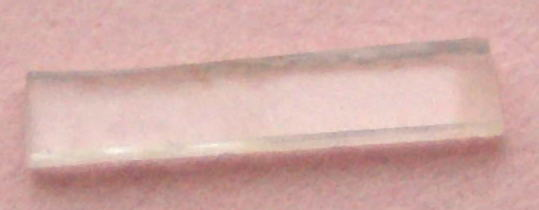
\includegraphics[width=\linewidth]{diagrams/GaNcrystal.jpg}
        \caption{Semiconductor GaN}
    \end{figure}
}    
\only<2>{
    \begin{figure}
        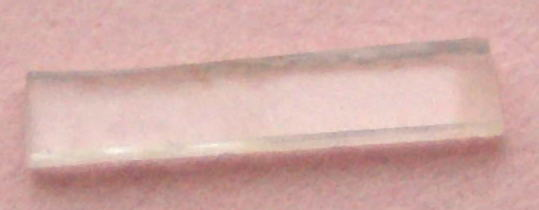
\includegraphics[width=\linewidth]{diagrams/GaNcrystal.jpg}
        \caption{Band Theory}
    \end{figure}
}
\only<3>{
    \begin{figure}
        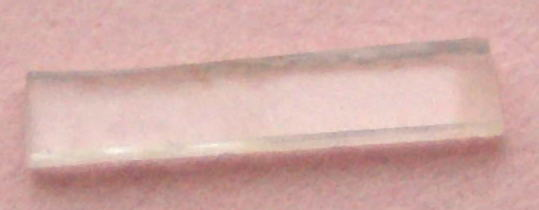
\includegraphics[width=\linewidth]{diagrams/GaNcrystal.jpg}
        \caption{Dirac Band Theory}
    \end{figure}
}
\only<4>{
    \begin{figure}
        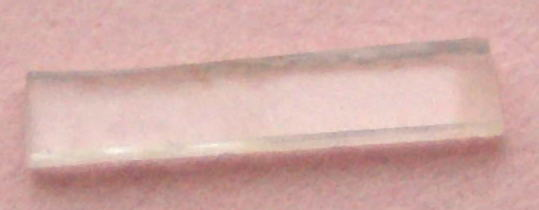
\includegraphics[width=\linewidth]{diagrams/GaNcrystal.jpg}
        \caption{Wannier Function}
    \end{figure}
}
\end{column}
\end{columns}
\end{frame}